\documentclass[12pt,a4paper,fleqn]{article}
\title{Progress Report}
\author{Syed Ahmad Raza}
\date{2017.03.28}
\usepackage{mathtools}
\usepackage{amsmath}
\usepackage{graphicx}
\usepackage{color}          % for color eps output
\usepackage{afterpage}
%\usepackage{layouts}       % for: \printinunitsof{in}\prntlen{\textwidth}

\begin{document}
\maketitle
\section*{Comparison of analytical and numerical solution of Laplace
equation using SOR method}

The following Laplace equation was considered:
\begin{equation}
\frac{\partial^2\phi}{\partial x^2} + \frac{\partial^2\phi}{\partial y^2} = 0
\end{equation}

The equation was discretized as follows:
\begin{equation}
\frac{\phi_{i+1,j}-2\phi_{i,j}+\phi_{i-1,j}}{(\Delta x)^2} +
\frac{\phi_{i,j+1}-2\phi_{i,j}+\phi_{i,j-1}}{(\Delta y)^2} = 0
\end{equation}

This equation can be re-arranged as follows:

\begin{equation}
\phi_{i,j} = \left(
\frac{\phi_{i+1,j}+\phi_{i-1,j}}{(\Delta x)^2} +
\frac{\phi_{i,j+1}+\phi_{i,j-1}}{(\Delta y)^2}
\right)\left(\frac{(\Delta x)^2(\Delta y)^2}{2[(\Delta x)^2+(\Delta y)^2]}\right)
\end{equation}

\subsection*{Jacobi Method}
For Jacobi method, the above equation would take the following form:
\begin{equation}
\phi^{m+1}_{i,j} =
\left(
\frac{\phi^m_{i+1,j}+\phi^{m}_{i-1,j}}{(\Delta x)^2} +
\frac{\phi^m_{i,j+1}+\phi^{m}_{i,j-1}}{(\Delta y)^2}
\right)\left(\frac{(\Delta x)^2(\Delta y)^2}{2[(\Delta x)^2+(\Delta y)^2]}
\right)
\end{equation}

\subsection*{Gauss-Seidel Method}
In Gauss-Seidel method, the values of $\phi$ are utilized as soon as they
are calculated and the equation takes the following form:
\begin{equation}
\phi^{m+1}_{i,j} =
\left(
\frac{\phi^m_{i+1,j}+\phi^{m+1}_{i-1,j}}{(\Delta x)^2} +
\frac{\phi^m_{i,j+1}+\phi^{m+1}_{i,j-1}}{(\Delta y)^2}
\right)\left(\frac{(\Delta x)^2(\Delta y)^2}{2[(\Delta x)^2+(\Delta y)^2]}
\right)
\end{equation}

\subsection*{SOR Method}
The equation changes for Successive Over-Relaxation method because of the
relaxation factor:
\begin{equation}
\phi^{m+1}_{i,j} = (1-\omega)\phi^m_{i,j} + \omega
\left(
\frac{\phi^m_{i+1,j}+\phi^{m+1}_{i-1,j}}{(\Delta x)^2} +
\frac{\phi^m_{i,j+1}+\phi^{m+1}_{i,j-1}}{(\Delta y)^2}
\right)\left(\frac{(\Delta x)^2(\Delta y)^2}{2[(\Delta x)^2+(\Delta y)^2]}
\right)
\end{equation}

This equation was solved using $\omega = 1.8$ for a $50\times50$ grid. The error
between the numerical solution and the exact solution is shown below in the
figure for various tolerance values.

\begin{figure}[p!]
\centering
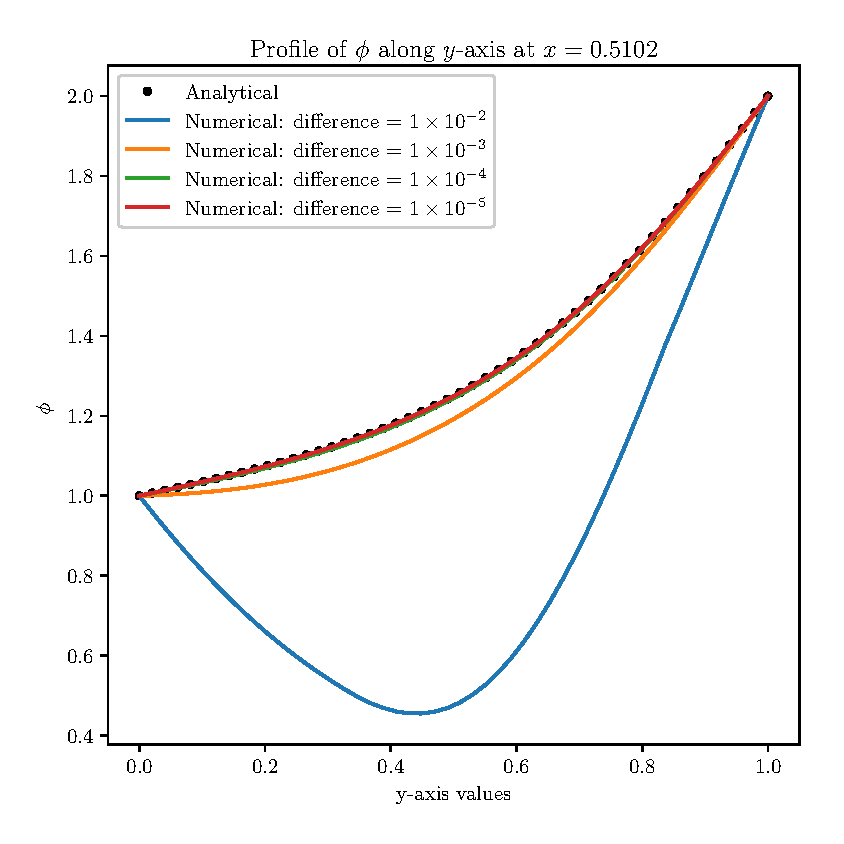
\includegraphics[width=\linewidth]{sorError.eps}
\caption{Comparison of numerical solution and exact solution of Laplace
equation for various runs of SOR method using different tolerance
(difference) values.}
\end{figure}

\end{document}